\documentclass{beamer}

\usetheme{Rochester}
\usecolortheme{material}
\usepackage{multicol}
\usepackage{listings}

\setbeamertemplate{footline}[text line]{%
  \parbox{0.5\linewidth}{
    \vspace*{-12pt} %\insertshorttitle~(\insertshortauthor)
  }
  \hfill%
  \parbox{0.5\linewidth}{
    \vspace*{-12pt}\raggedleft\insertpagenumber
  }
}
\lstset{
breaklines=true, 
basicstyle=\scriptsize, 
keywordstyle=\color{blue700},
basewidth=0.55em
}
\setbeamertemplate{navigation symbols}{}
\begin{document}
\title[Entwurssprachen]{HW/SW Entwurfssprachen am Beispiel System-C}
\author[Zaruba F., Weber T.]{Florian Zaruba, Thomas Weber}
\date{\today} 

\begin{frame}
\titlepage
\end{frame}

\begin{frame}\frametitle{Table of contents}
%\begin{multicols}{2}
  \tableofcontents
%\end{multicols}
\end{frame}

\note{Everything you want}

\section{HW/SW Design Languages} 

\begin{frame}\frametitle{Motivation} 

\begin{itemize}
	\item Rapidly increasing number of embedded systems.
\end{itemize}
\pause
	    \begin{figure}[hp]
		  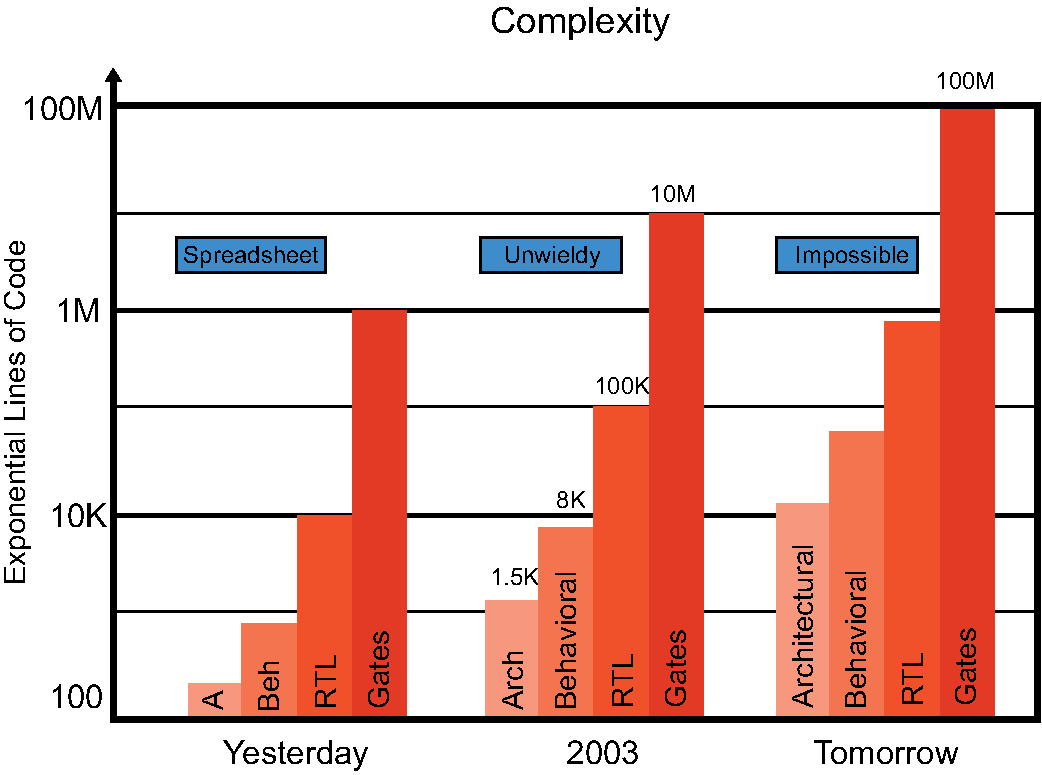
\includegraphics[width=0.6\textwidth]{pictures/complexity.pdf}
	      \caption{Increasing complexity \cite{black2004systemc}}
	      \label{fig:flow}
	    \end{figure} 
\end{frame}

\begin{frame}\frametitle{System-Level Description Language (SDL)} 
\begin{itemize}
	\item Specification and design at various abstraction levels
	\item Faster design cycles %? 
	\item Seperation between communication and functionality (TLM)
	\item e.g.: SystemC (by accellera systems initiative), System Verilog, SpecC
\end{itemize}
\end{frame}

\section{SystemC Overview}
\begin{frame}\frametitle{What is SystemC}
\begin{itemize}
	\item Set of C++ classes and macros (Concurrency and notion of time)
	\item Common language for SW and HW, C++
	\item Enhanced productivity, support higher abstraction level (TLM)
	\item Many C++ libraries useful
\end{itemize}
\end{frame}

\begin{frame}\frametitle{SystemC Architecture}
    \begin{figure}[hp]
	  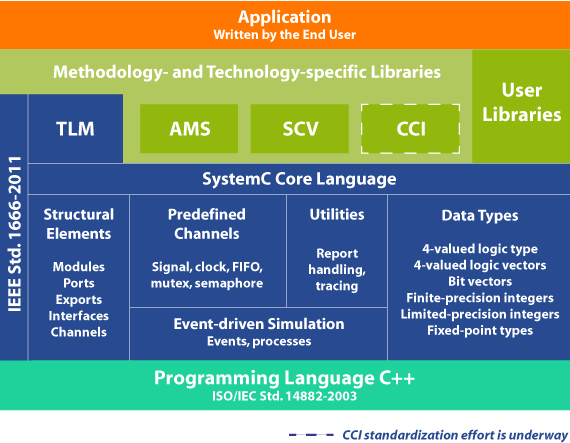
\includegraphics[width=0.70\textwidth]{pictures/systemc-architecture}
      \caption{SystemC architecture \footnote{\url{http://www.accellera.org/community/systemc/about_systemc/}}}
      \label{fig:flow}
    \end{figure}
\end{frame}

\subsection{History}
\begin{frame}\frametitle{History} 
\begin{itemize}
	\item 27/09/1999 Open SystemC Initiative announced
	\item 01/03/2000 V0.91 released
	\item 01/02/2001 V2.0 released
	\item 06/06/2005 SystemC 2.1 LRM and TLM 1.0 released
	\item 12/07/2006 SystemC Verification Library 1.0p2
	\item 09/06/2008 TLM-2.0.0 library released
	\item 08/03/2010 SystemC AMS extension 1.0 released
	\item 10/11/2011 IEEE pproves the IEEE 1666–2011 standard for SystemC
	\item Currently SystemC V2.3.1, AMS 2.0, SystemC Verification 2.0
\end{itemize}
\end{frame}


\begin{frame}\frametitle{Where does it fit in?} 
	    \begin{figure}[hp]
	      \centering
	      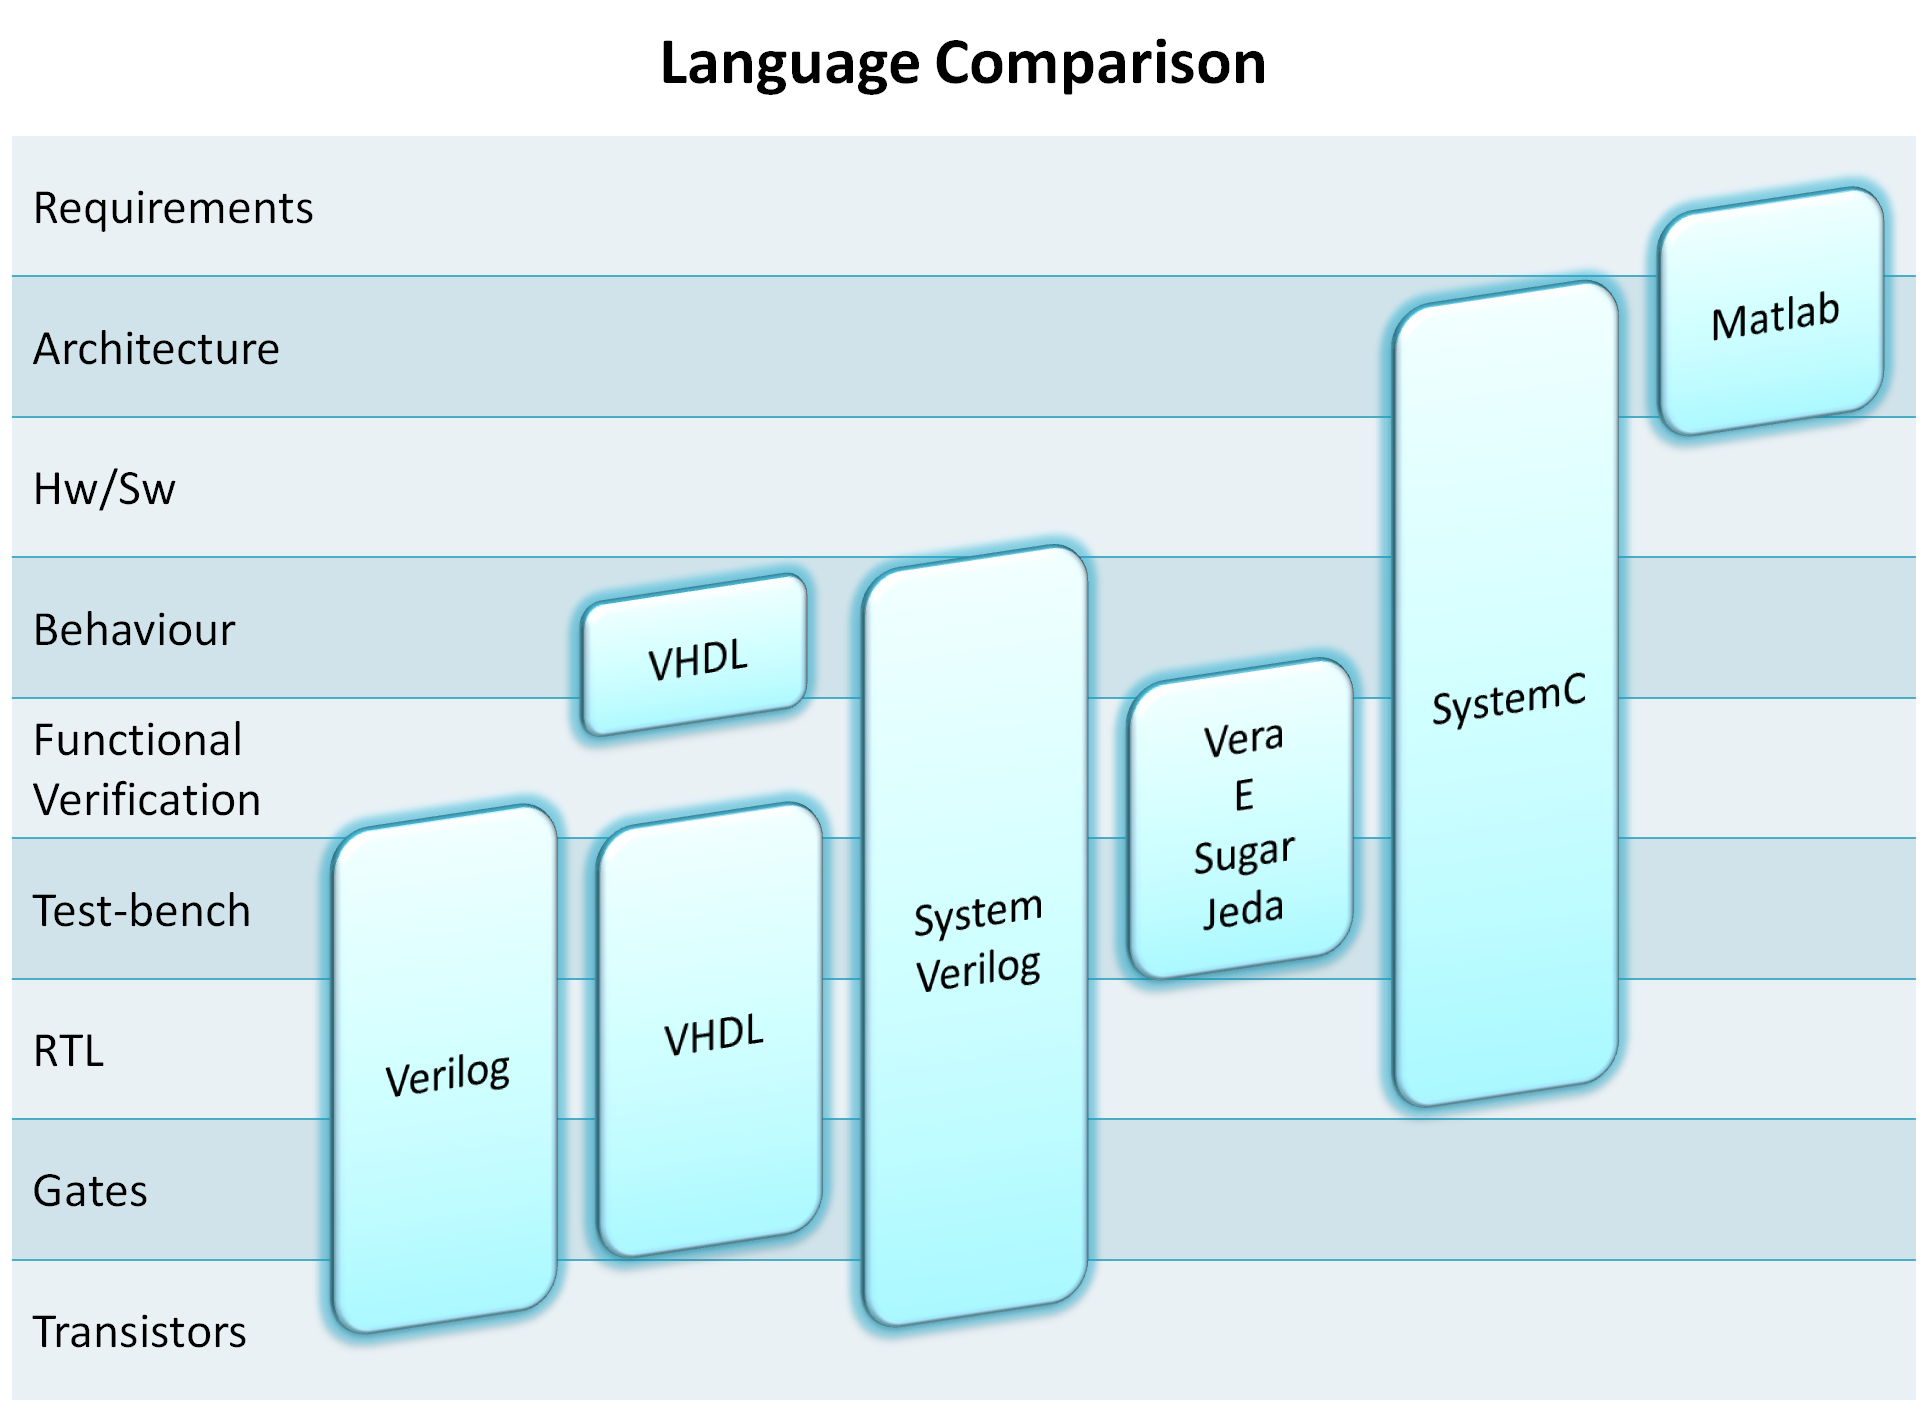
\includegraphics[width=0.7\textwidth]{pictures/Hardware_Description_Languages_and_Abstraction_Levels.png}
	      \caption{Hardware Description Languages and Abstraction Levels\footnote[frame]{\url{http://www.esa.int/Our_Activities/Space_Engineering/Microelectronics/System-Level_Modeling_in_SystemC}}}
	      \label{fig:flow}
	    \end{figure} 

\end{frame}

\subsection{Benefits/Drawbacks}
\begin{frame}\frametitle{Benefits/Drawbacks} 
\begin{itemize}
	\item Benefits
	\begin{itemize}
		\item Lots of C++ libraries available and useful
		\item IEEE standard
		\item Virtual prototyping
		\item Verification
	\end{itemize}
	\item Drawbacks \begin{itemize}
		\item Still a C++ compiler/runtime errors
		\item Debug C++, not System-C
	\end{itemize}
\end{itemize}
\end{frame}


\subsection{Features of SystemC}
\begin{frame} \frametitle{Features of SystemC} 
  \begin{itemize}
   \item C
    \begin{itemize}
      \item{notion of time}
      \item{hardware datatypes}
    \end{itemize}
   \item VHDL
    \begin{itemize}
      \item{verification}
      \item{complexity}
    \end{itemize}
   \item SystemC Features
    \begin{itemize}
      \item{Modules}
      \item{Processes/Threads}    
      \item{Ports and Signals}
      \item{Time}
    \end{itemize}
  \end{itemize}
\end{frame}

\subsection{Examples - Comparison}
\begin{frame}[fragile] \frametitle{C vs. SysC vs. VHDL Datatypes} 
\begin{tabular}{p{0.27\textwidth}|p{0.31\textwidth}|p{0.36\textwidth}}
\multicolumn{1}{c}{\textbf{C}} & \multicolumn{1}{c}{\textbf{SystemC}} & \multicolumn{1}{c}{\textbf{VHDL}} \\
\begin{lstlisting}[language=C]
bool
char
uintk_t
int 
long
...
\end{lstlisting}
& 
\begin{lstlisting}[language=C++, ]
sc_bit
sc_logic
sc_lv[k]
sc_uint<k>
sc_signal<...>
\end{lstlisting}
 &  
\begin{lstlisting}[language=VHDL]
bit
std_logic
std_logic_vector (k dowto 0)
signal
\end{lstlisting}
\end{tabular}

\end{frame}

\begin{frame}[fragile] \frametitle{C vs. SysC vs. VHDL Architecture} 
\begin{tabular}{p{0.27\textwidth}|p{0.31\textwidth}|p{0.36\textwidth}}
\multicolumn{1}{c}{\textbf{C}} & \multicolumn{1}{c}{\textbf{SystemC}} & \multicolumn{1}{c}{\textbf{VHDL}} \\
\begin{lstlisting}[language=C,basicstyle=\tiny]
/* c - header*/

bool sample_module(bool clk, bool reset, bool enable)
{
  //timefunction?
  if(reset == false){
    a = true;
  }
}
\end{lstlisting}
& 
\begin{lstlisting}[language=C++,basicstyle=\tiny]
  SC_MODULE(sample_module){
    sc_in_clk	  clk;//clock
    sc_in<sc_bit> reset;//signals
    sc_in<sc_bit> enable;
    sc_out<sc_bit> a;	//output
        
    void a_function(){      
      if(reset.read() != 0){
        a.write('1');	
      }
      
     SC_CTOR(){
       SC_METHOD(a_function);
       sensitive_pos << clk; 
       //sensitive << clk.pos();
     }
      
    }
  }
  
\end{lstlisting}
 &  
\begin{lstlisting}[language=VHDL,basicstyle=\tiny]
architecture sample_arch of sample_module is

   clk : in std_logic;
   reset : in std_logic;
   enable: in std_logic;
   a	: out std_logic;
   
  begin
  
  a_function : process(clk)
  begin
  if reset = '1' then
    a <= '1';
  end if;
  
end architecture ;

\end{lstlisting}
\end{tabular}
\end{frame}

\subsection{Examples - Question}
\begin{frame}[fragile]\frametitle{SystemC Quizz} 
SystemC Codesample.
\begin{lstlisting}[language=C++,basicstyle=\tiny]
#include "systemc.h"
SC_MODULE (first_prog) {
  sc_in_clk     clock ;      // Clock input of the design
  sc_in<bool>   reset ;      // active high, synchronous Reset input
  sc_in<bool>   enable;     
  sc_out<sc_uint<4> > output;
  sc_uint<4>	something;
  void incr_something () {
    if (reset.read() == 1) {
      something =  0;
      output.write(something);
    } else if (enable.read() == 1) {
      something = something + 1;
      output.write(something);
      cout<<"@" << sc_time_stamp() <<" :: Incremented Something "
        <<output.read()<<endl;
    }
  }
  SC_CTOR(first_prog) {
    cout<<"Executing new"<<endl;
    SC_METHOD(incr_something);
    sensitive << reset;
    sensitive << clock.pos();
  }
};
\end{lstlisting}
AND-Gatter? OR-Gatter? Counter? FlipFlop?
\end{frame}

\section{Partitioning}
\begin{frame}\frametitle{Partitioning} 
	    \begin{figure}[hp]
	      \centering
	      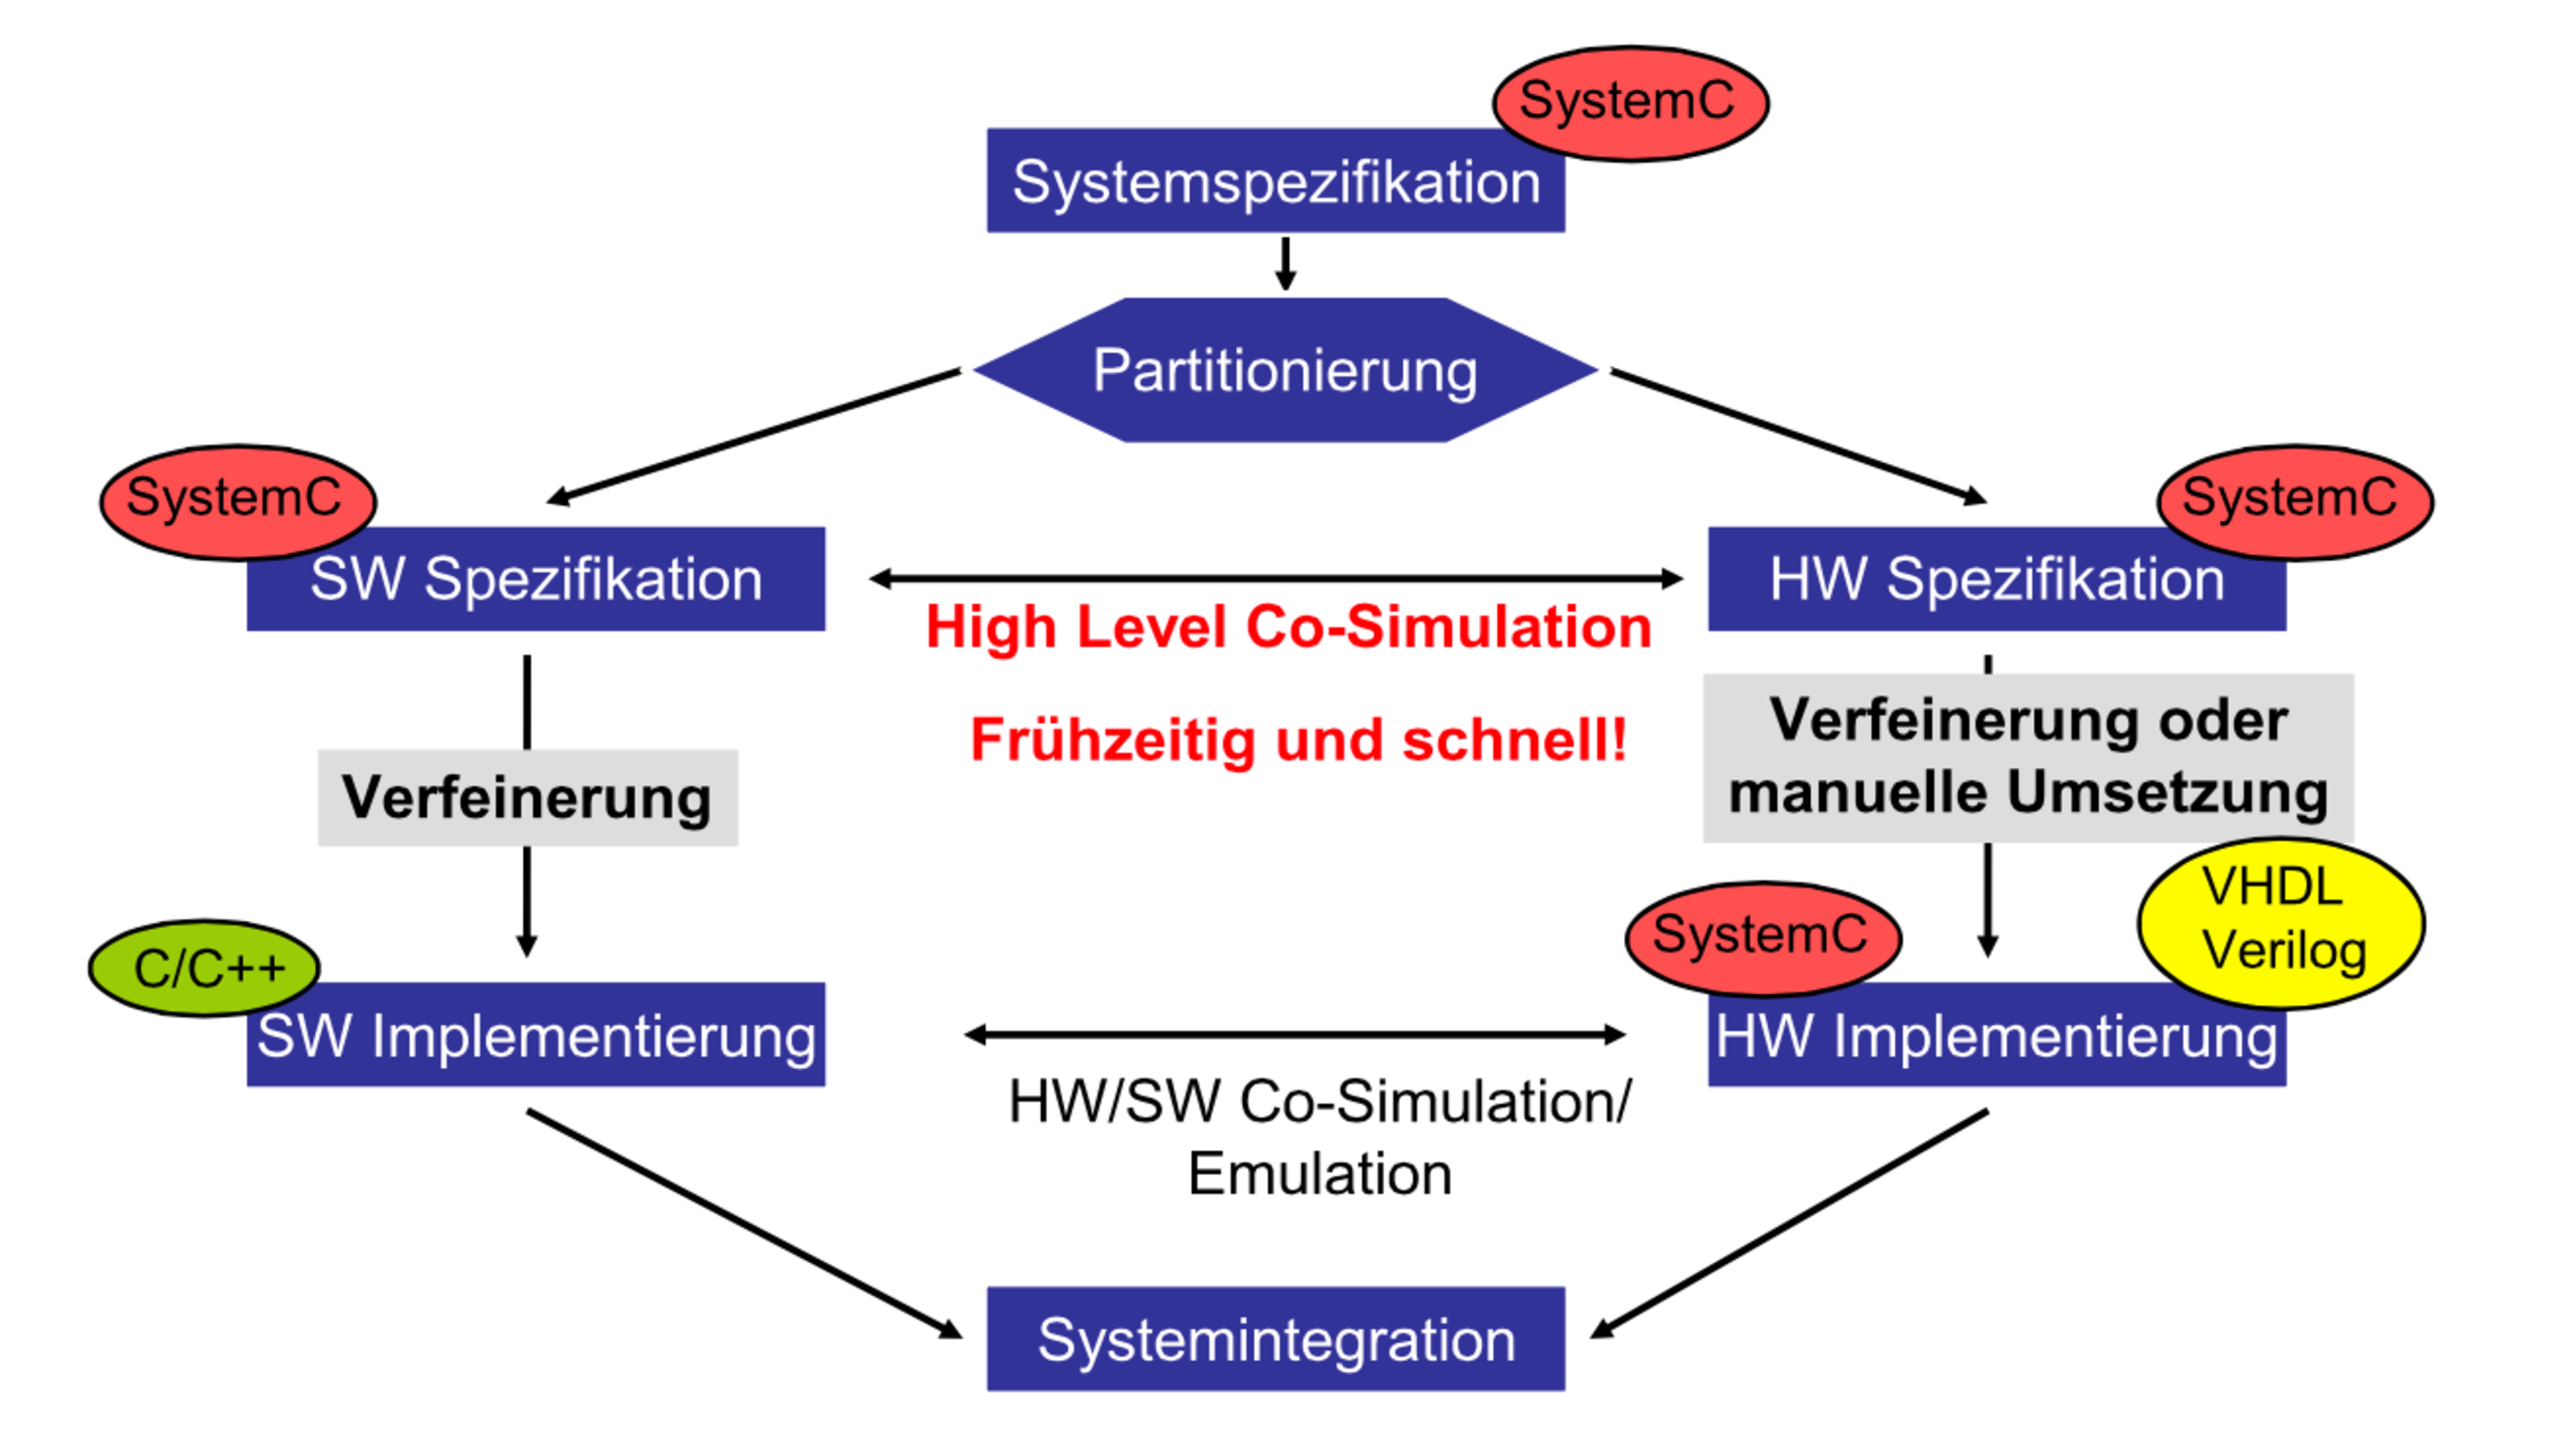
\includegraphics[width=1.0\textwidth]{pictures/design_flow.pdf}
	      \caption{Partitioning of HW and SW \cite{braunschweig}}
	      \label{fig:flow}
	    \end{figure} 
%\begin{block}{title of the bloc}
%bloc text
%\end{block}

%\begin{exampleblock}{title of the bloc}
%bloc text
%\end{exampleblock}


%\begin{alertblock}{title of the bloc}
%bloc text
%\end{alertblock}
\end{frame}


\section{Automated Partitioning}
\begin{frame}\frametitle{Automated Partitioning} 

\begin{itemize}
  \item Techniques
  \begin{itemize}
   \item Partitioning Algorithms (Graph Theory)
    \begin{itemize}
      \item{Kernighan-Lin-Algorithm}
      \item{Simulated annealing}  
    \end{itemize}
   \item Design Space Exploration
  \end{itemize}
  
  \item{Tools}
    \begin{itemize}
   \item{LegUP - Open Source}
    \end{itemize}
 \end{itemize}
\end{frame}


\section{SystemC Tools}
\begin{frame}\frametitle{SystemC Tools} 
\textbf{SystemC to VHDL}
    \begin{itemize}
      \item{gcc/gdb for simualtion/debugging}
      \item{Catapult SL/LP}
      \item{Cynthesizer 5}
      \item{Modelsim - Verification}
      \item{Bambu - Open Source (C behavioral desc.)}
      \item{Mentor Graphics Catapult C/Mentor Graphics System Vision}
      \item{Cadence C-to-Silicon Compiler}
      \item{Xilinx Vivado Design Suite}
    \end{itemize}
\end{frame}

\section{Who uses it?}
\begin{frame} \frametitle{Users} 
    \begin{itemize}
      \item{ARM Ltd.}
      \item{AMD}
      \item{Intel}
      \item{Futjitsu VSLI}
      \item{STMicroelectronics}
      \item{Realtek}
      \item{...}
    \end{itemize}
\end{frame}
      
\section{Bibliography}
\nocite{haubelt2010digitale}
\nocite{canis2011legup}
\nocite{liao2002system}
\nocite{initiative2014functional}
\begin{frame}[allowframebreaks] \frametitle{Literature} 
\bibliographystyle{plain}
\bibliography{references}
\end{frame}



\end{document}
